\chapter{Stand der Technik / Systemkonzept}
Dieses Kapitel ist stark davon abh�ngig welche Art von Arbeit beschrieben werden soll. Bei einer Projektdokumentation sind hier die Grundlagen in rudiment�rer Form anzugeben und ein Systemkonzept zu entwickeln. F�r das Erstellen einer Bachelor und Master Thesis sind die Abschnitte \enquote{Stand der Technik} und \enquote{Grundlagen} zwingend vorgegeben. Der Abschnitt \enquote{Systemkonzept} ist abh�ngig von der Aufgabenstellung und nicht immer notwendig f�r eine Bachelor und Master Thesis.


%---------------------------------------------------------
\section{Stand der Technik (Bachelor, Master)}
Anhand der Aufgabenstellung ist der \enquote{Stand der Technik}\footnote{State of the Art} zu ermitteln. Hierunter wird die Aufarbeitung der Literatur zum allgemeinen Problemumfeld und insbesondere zu der speziellen Fragestellung der Arbeit verstanden. Hierzu sind Literaturrecherchen in einschl�gigen Datenbanken (IEEE-Publikationen, ACM\footnote{Association for Computing Machinery} Digital Library, Science Direct College Edition, SpringerLink, Academic Search Elite, Datenbankportal (DBIS), ...) durchzuf�hren und allgemeine Internetrecherchen. Es sind folgende Fragen zu beantworten:
\begin{itemize}
  \item Welche Ans�tze gibt es bereits?
  \item Wie beurteilen verschiedene Autoren die Ans�tze?
  \item Was sind relevante Standards oder etablierte Vorgehensweisen?
  \item Welche Fragestellungen der Arbeit werden in der Literatur nicht behandelt?
\end{itemize}
%---------------------------------------------------------
\section{Grundlagen (Bachelor, Master)}
Grundlagen sind nicht in jeder Arbeit n�tig und k�nnen unterschiedlich umfangreich ausfallen. Im Wesentlichen gilt hier: sie sollten nur das enthalten, was sp�ter im Verlauf der Arbeit tats�chlich ben�tigt wird. Trivialit�ten sind nicht darzustellen. Besonders wichtig ist es hier alle Aussagen, Erkl�rungen und Beschreibungen durch passende Referenzen (Literaturverweise \verb!\ref{...}! an den entsprechenden Stellen zu st�tzen.

%---------------------------------------------------------
\section{Systemkonzept (Projekt)}
Anhand der Aufgabenstellung ist hier ein Konzept f�r die L�sung der Aufgabe zu erstellen. Startpunkt sollte ein Blockschaltbild sein. Die Komponenten des Blockschaltbildes sind im Detail zu beschreiben. Hieraus sind Eigenschaften der notwendigen Hard- und Software abzuleiten.
Als Werkzeug f�r die Erstellung ist das Programm VISIO 2007 von Microsoft zu verwenden. Abbildung \vref{fig:blockschaltbild} zeigt exemplarisch ein einfaches Blockschaltbild eines embedded System.
\begin{figure}[htbp]
	\centering
		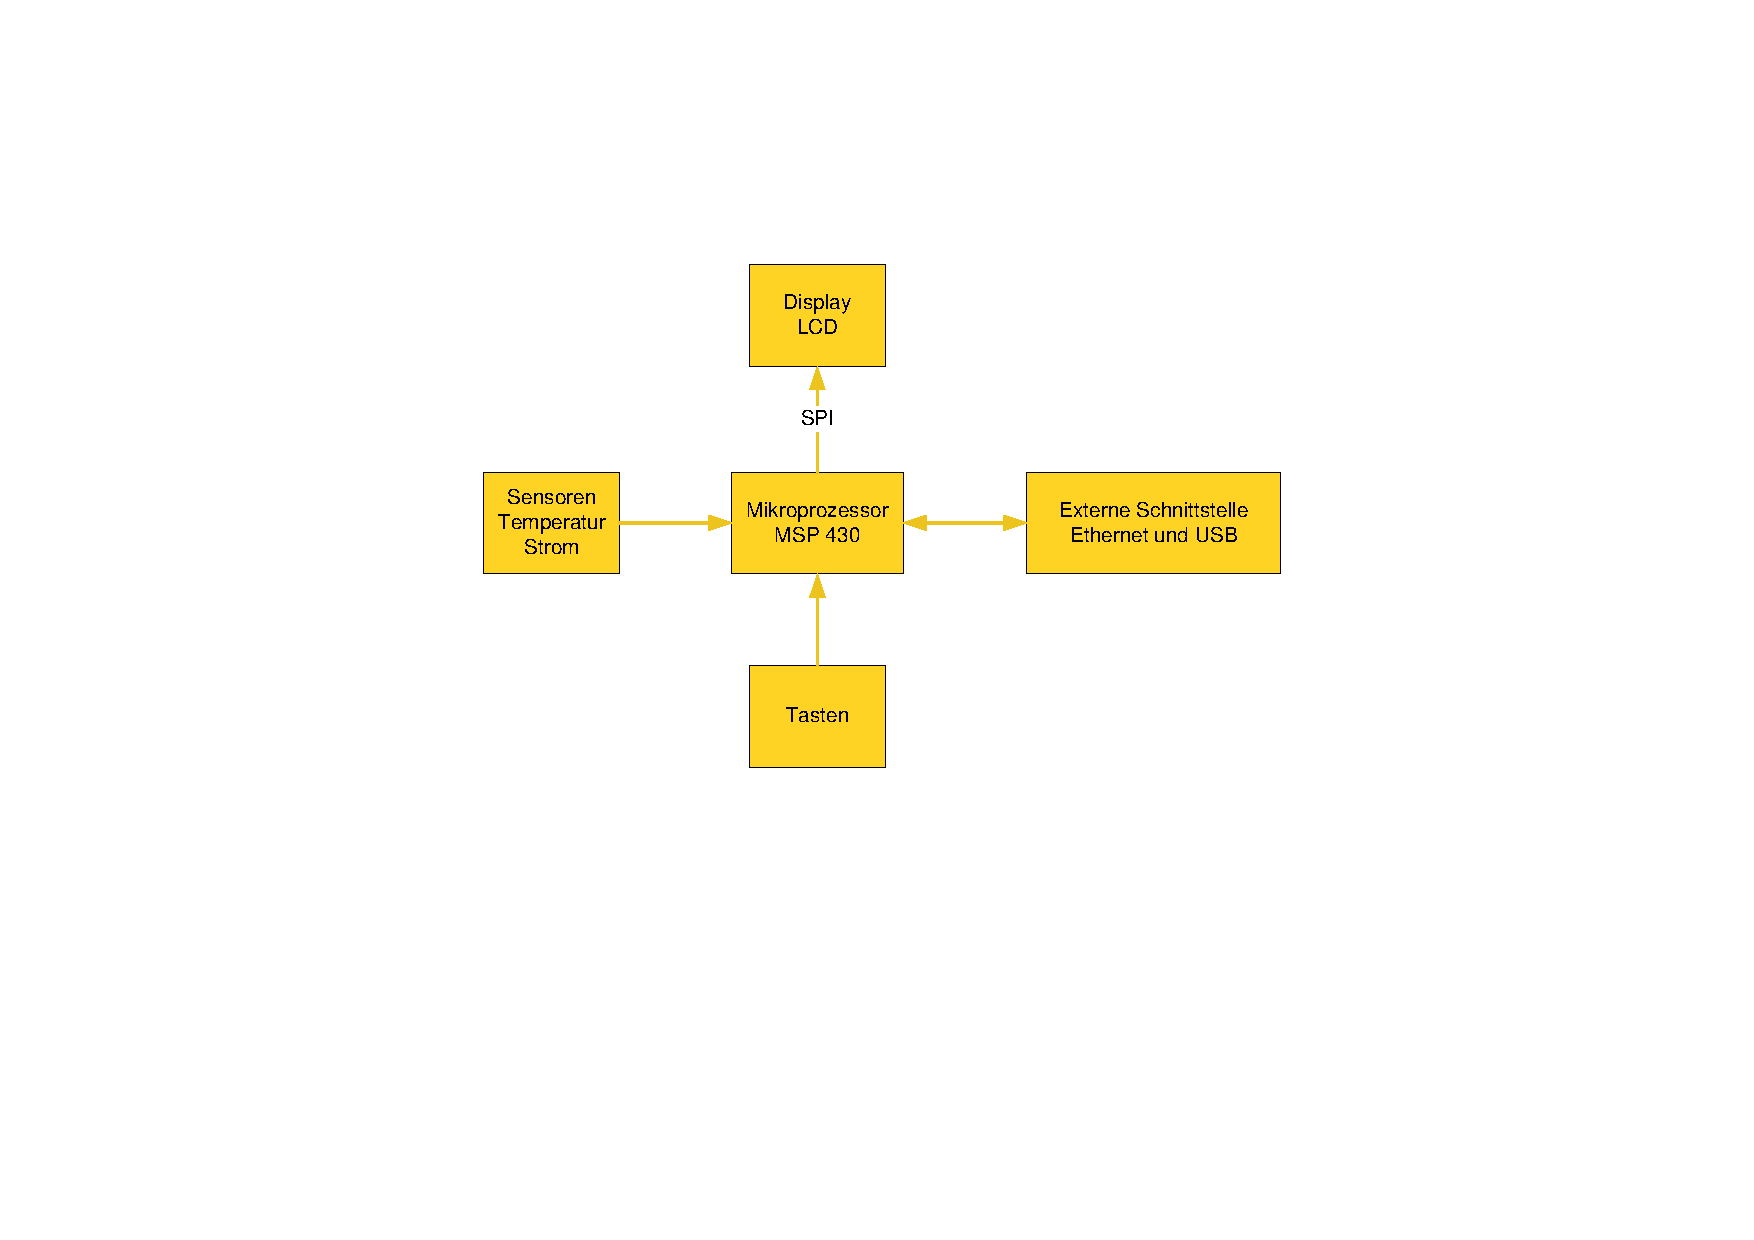
\includegraphics[width=0.8\textwidth]{Bilder/Blockschaltbild.pdf}
	\caption{Beispiel eines Blockschaltbildes}
	\label{fig:blockschaltbild}
\end{figure}
